\section{Lezione 21}%
\label{sub:Lezione 21}
\subsection{K.S. Entropy}%
\label{sub:K.S. Entropy}
Prendiamo un sistema dinamico come una mappa Hamiltoniana che conserva una certa misura su un insieme $X$.\\
Supponiamo di introdurre una partizione di $X$ chiamata $Q$ tale per cui non ci sono sovrapposizioni tra le partizioni $Q_i$.\\
Inoltre chiediamo una ipotesi più forte: un punto $x\in X$ che appartiene ad uno solo dei $Q_i$ e vi appartiene anche ogni sua $n$-esima iterata della mappa $T$.\\
Possiamo costruire una dinamica simbolica: una sequenza di interi $\left\{x_n\right\}$ tali che:
\[
    T^nx \in Q_{x_n}
.\] 
Si dice \textbf{partizione generatore} la partizione $Q$ se per ogni $x$ si ha una unica dinamica simbolica (quindi una unica sequenza di interi).
\subsubsection{Strumento per definire l'entropia: Baker Trasformation}%
\label{subsub:Applicazione: Baker Trasformation}
Prendiamo un sistema bidimensionale con variabili $p,q$, la trasformazione di Baker ha la seguente forma:
\[
    T(p,q)=
    \begin{cases}
	2p ,\  q /2 \qquad &\text{se } 0 \le p < 1 /2\\
	2p-1, \ q /2 + 1 /2 \qquad &\text{se } 1 /2 \le p \le 1
    \end{cases}
\]
\begin{figure}[H]
    \centering
    \incfig{21_baker}
    \caption{\scriptsize Passaggi operativi della mappa di Baker. Si fa come con il pane: si mette sopra e poi si schiaccia.}
    \label{fig:21_baker}
\end{figure}
\noindent
Con questa mappa è comodo scrivere le coordinate $p,q$ in base 2:
\[
    p = \sum_{k=0}^{-\infty} s_k 2^{k-1} \qquad q = \sum_{k=1}^{\infty} s_k 2^{-k}
.\] 
Le potenze $k$ dello sviluppo sono negative, questo perché le variabili vanno da $0$ a $1$. Le $s_k$ inoltre possono valere $0$ o $1$.\\
Ogni punto in questa base è esprimibile come sequenza di $0$ e $1$ nel seguente modo:
\begin{equation}
    x_i = \left(\ldots, s_{-2}, s_{-1}, s_0, s_1, \ldots\right)
    \label{eq:21_baker_list}
\end{equation}
Vediamo come agisce la mappa con un esempio pratico: se si ha $0<p< 1 /2$ e si applica $T$ avremmo che 
\[
    p\to 2p, \qquad q \to q /2
.\] 
Nel linguaggio della lista dei $s_i$ questo significa che tutti gli $s_i$ andranno verso destra. Quindi l'evoluzione della mappa è semplicemente lo spostare i coefficienti $s_i$ verso destra con la notazione \ref{eq:21_baker_list}.\\
Abbiamo anche un effetto di bordo tra le $p$ e le $q$: $s_0$ perchè dovrebbe andare in $s_1$ visto che il primo è un fattore di $p$ e l'altro è un fattore di $q$?\\
La risposta è proprio nella natura della trasformazione che "ruota" lo spazio $p$ e $q$. Facendo un controllo nel caso specifico patologico ($p=1/2$) si vede subito che il coefficiente $s_0$ deve necessariamente andare in $s_1$.\\
\subsubsection{Definizione di KS entropy}%
\label{subsub:Definizione di KS entropy}
Introduciamo adesso la partizione che deriva dalla intersezione delle iterate della trasformazione di Baker.
\begin{figure}[H]
    \centering
    \incfig{21_def_E}
    \caption{\scriptsize Mappa di Baker con intersezione delle partizioni.}
    \label{fig:21_def_E}
\end{figure}
\noindent
Potremmo iterare la procedura più volte ottenendo ogni volta una potenza di due in più nel numero di partizioni.\\
Si definisce  KS Entropy:
\[
h_{_{KS}} = \text{sup}\left( \lim_{n \to \infty} \frac{h\left[ AV(TA)V(T^2A)V\ldots VT^{n-1}A\right]}{n}\right)
.\] 
con 
\[
    h(A)=-\sum_{i}^{} p_i\ln (p_i)
.\] 
Dove $p_i$ è l'area della partizione $i$.\\
Nel caso della mappa di Baker si ha che il numero di partizioni generate alla $n$-esima iterazione (considerando anche l'operatore di intersezione $V$) è $2^{n}$. L'area di ogni partizione sarà allora $2^{-n}$ e l'entropia di KS vale:
\[
    h_{_{KS}} = \frac{1}{n}\sum_{i}^{2^{n}} \left(\frac{1}{2^{n}}\right)n\ln\left(\frac{1}{2}\right) = \ln 2
.\] 
Sempre nel caso della Baker trasform. proviamo a calcolare gli esponenti di Lyapunov: 
\[
    \begin{pmatrix} p \\ q \end{pmatrix}_{n+1} = 
    \begin{pmatrix} 
	2 & 0 \\
	0 & 1/2
    \end{pmatrix} 
    \begin{pmatrix} p \\ q \end{pmatrix}_n
.\] 
Si vede subito che gli autovalori in questione sono:
\[
    \lambda_1 = 2 \qquad \lambda_2 = 1 /2
.\] 
Quindi gli esponenti di Lyapunov per la mappa sono $\pm \ln 2$. Il più grande tra i due esponenti è proprio l'entropia di KS, è un caso?
\begin{redbox}{Teorema di Piesin}
    La KS entropy è la somma degli esponenti di Lyapunov positivi.
    \[
        h_{_{KS}} = \int_{P}^{} \sum_{\lambda_i >0}^{} \lambda_id\mu 
    .\] 
    In cui $\lambda_i$ sono gli esponenti di Lyapunov in una regione di energia $E$ di misura $d \mu$.
\end{redbox}
\noindent
\subsection{Indicatori di Caos globale}%
\label{sub:Indicatori di Caos globaliIndicatori di Caos globale: metodo di Chirinkov}
\subsubsection{Metodo di Chirinkov}%
\label{subsub:metodo di Chirinkov}
L'idea alla base per trovare il caos globale è quella di cercare, anziché le singole traiettorie caotiche, delle intere strutture caotiche nello spazio delle fasi.\\
Partiamo da un sistema Hamiltoniano integrabile perturbato:
\[
    H(I,\theta) = H_0(I) + \epsilon H_I(I, \theta)
.\] 
Scriviamo la perturbazione in componenti spettrali di Fourier:
\[
    H(I,\theta) = H_0(I) + \epsilon \sum_{m}^{} H_m(I)e^{im\theta}
.\] 
Sappiamo che la mappa per l'Hamiltoniana imperturbata è la seguente:
\[
    \begin{cases}
	I_i = I_i(0)\\
	\theta_i = \omega_i(I)t + \theta_i(0)
    \end{cases}
.\] 
Con la pulsazione $\omega$ che è definita da:
\[
    \omega_i = \frac{\partial H_0}{\partial I_i} 
.\] 
Inseriamo la perturbazione e ipotizziamo che questa abbia una sola componente spettrale:
\[
    H(I,\theta) = H_0(I) + \epsilon H_m(I)e^{im\theta}
.\] 
Allora abbiamo visto che:
\[\begin{aligned}
    &\dot{I}_i = -i \epsilon  m_i H_m(I)e^{im\theta}\\
    &\dot{\theta}_i = \omega_i(I) + \epsilon  H'_m(I)e^{im\theta}
.\end{aligned}\]
E all'ordine $\epsilon$  la soluzione è:
\[
    I_i = I_i(0)-\frac{\epsilon m_i H'_m(I_0)e^{i(m\cdot \omega)t + i\delta}}{m\cdot \omega}
.\] 
La trasformazione canonica "astuta" che permette di rendere integrabile l'Hamiltoniana al primo ordine in $\epsilon$ in questo caso è:
\[
    F = m_{\perp}I
.\] 
Dove $m_{\perp}$ è tale per cui $m_{\perp}\cdot m = 0$. In tal caso la trasformazione canonica elimina la risonanza.\\
Questo metodo funziona quando abbiamo una sola risonanza, con più risonanze non è possibile "curare" il sistema: la teoria perturbativa non risolve in tutto lo spazio con più risonanze.\\
Visivamente il caos arriva quando si hanno sistemi nello spazio delle fasi del tipo:
\begin{figure}[H]
    \centering
    \incfig{21_risonanze}
    \caption{\scriptsize Spazio delle fasi in presenza di due risonanze: quando i lobi si avvicinano iniziano a rompersi i tori e a quel punto siamo in presenza di un caos globale.}
    \label{fig:21_risonanze}
\end{figure}
\begin{exmp}[Mappa standard]
    Nel caso della mappa standard si ha:
    \[\begin{aligned}
	H(I, \theta, t) =& \frac{I^2}{2} + 2\pi k \cos\theta  \sum_{m = -\infty}^{\infty} \delta (2\pi m-t) = \\
	=& \frac{I^2}{2} + k \sum_{n= -\infty}^{\infty} \cos (\theta-nt)
    .\end{aligned}\]
    La mappa che abbiamo visto nelle lezioni precedenti è proprio questa integrata su un periodo.\\
    Vediamo che in questo caso generale escono fuori dei termini del tipo:
    \[
	H^{(n)}=\frac{I^2}{2}+k \cos\psi_n \qquad \psi_n = \theta-nt
    .\] 
    Abbiamo un set di Hamiltoniane risonanti con 
    \[
        \omega_n \equiv n
    .\] 
    Possiamo trovare la larghezza dell'"occhio" $\Delta\omega$ valutando la $I$ nel minimo del potenziale periodico:
    \[
        0 = \frac{I^2}{2}-k \implies  \Delta\omega_n \equiv I_{\text{max}, n} = 2\sqrt{k} 
    .\] 
    Come abbiamo detto in precedenza le $\omega$ sono numeri interi $n$, quindi tra una risonanza e l'altra c'è una distanza unitaria.\\
    Per questo motivo possiamo affermare che i lobi iniziano a toccarsi quando la loro distanza vale $1$, se due lobi distano tale valore significa che la larghezza del singolo occhio vale $1 /2$:
    \[
        \frac{1}{2} = 2k^{1 /2} \implies  k = \frac{1}{16}
    .\] 
    Per tale valore di $k$ (e per valori minori) nel sistema si ha una forma di caos globale. Possiamo verificare la cosa andando a setacciare la mappa standard al variare di $k$:
    \begin{figure}[H]
        \centering
	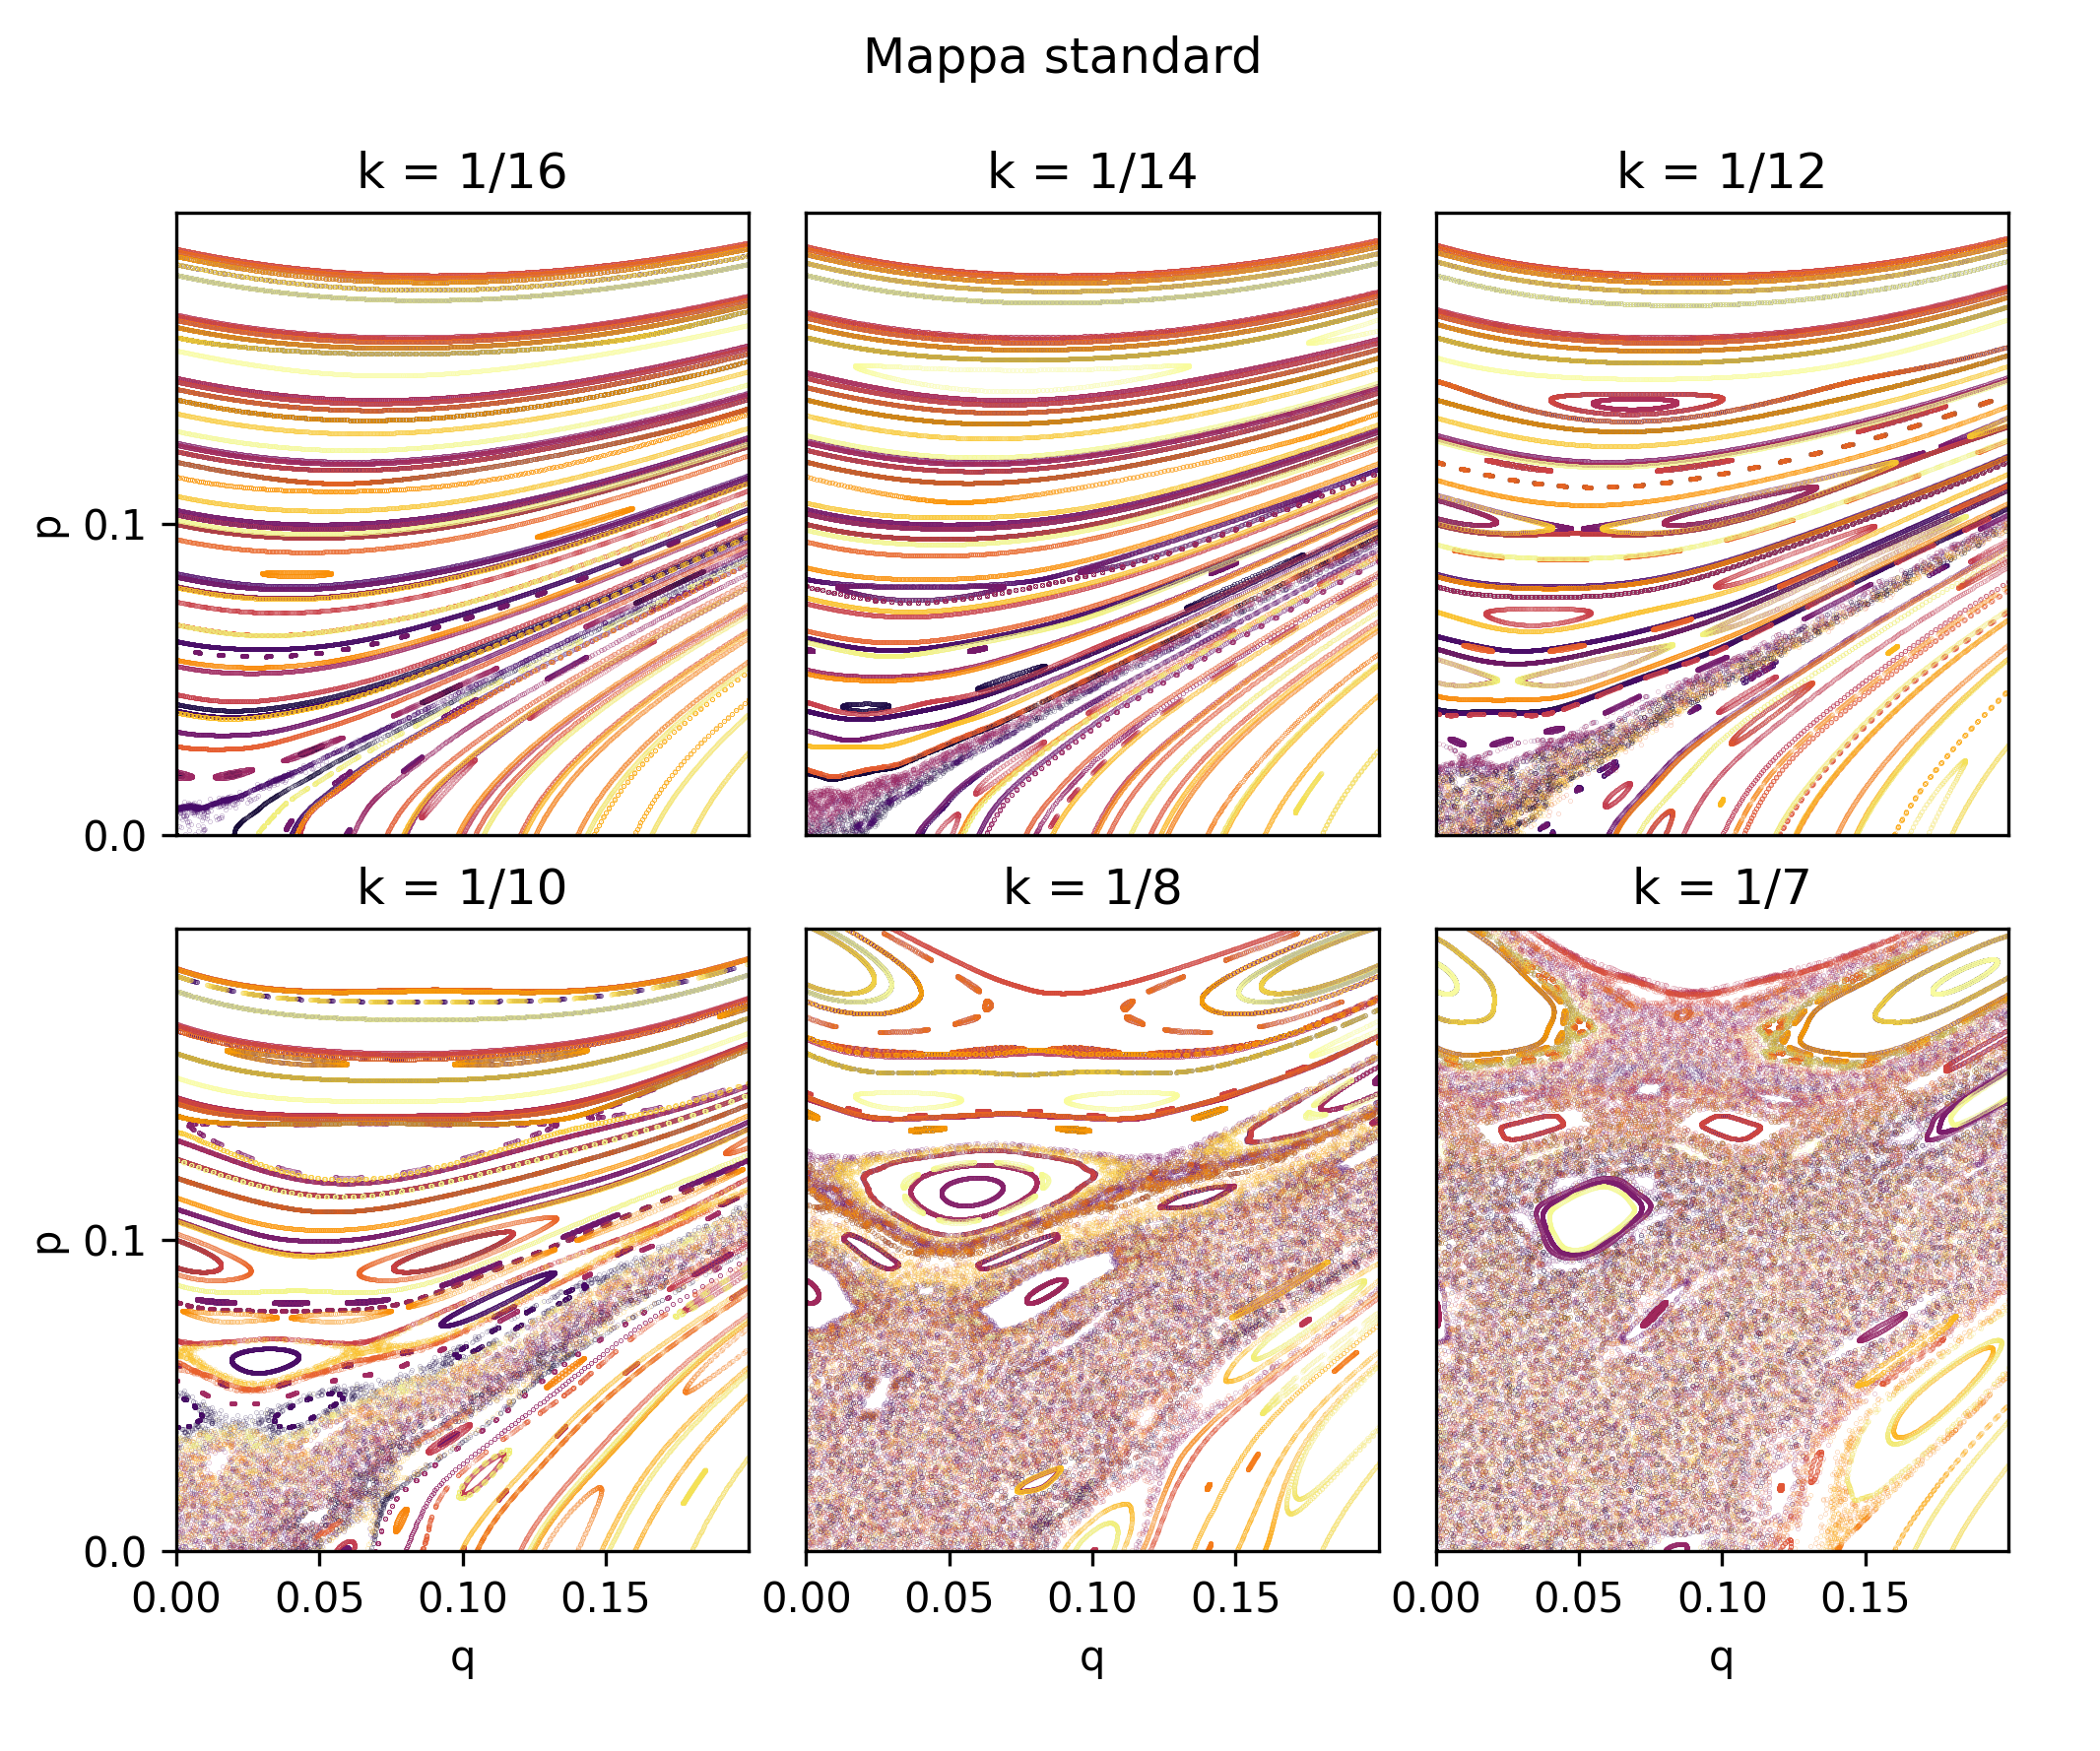
\includegraphics[width=0.47\textwidth]{figures/21_standard_maps.png}
        \caption{\scriptsize Zoom della mappa standard: si usano gli stessi parametri iniziali per tutte le traiettorie e si fa variare $k$ nella mappa.\\
	i primi cenni di caos in basso a sinistra (in tutte le figure) si hanno per $k = 1 / 16$.}
        \label{fig:figures-21_standard_maps-png}
    \end{figure}
\end{exmp}
\noindent
\begin{exmp}[Sistema di Henon-Hieles]
    Questo esempio è un ripasso della teoria perturbativa ed una applicazione al criterio di Chirinkov.\\
    Prendiamo la seguente Hamiltoninana con perturbazione:
    \[
        H = \frac{q_x^2+q_y^2}{2} + \frac{p_x^2+p_y^2}{2} + \epsilon q_x^2q_y^2
    .\] 
    La trasformazione canonica per le variabili azione angolo ci conduce a:
    \[
        H_0 = \omega_xI_x + \omega_yI_y
    .\] 
    Riscriviamo anche la trasformazione canonica inversa per completezza, come sempre:
    \[
        \begin{cases}
            q_x =\sqrt{2I_x} \cos\theta_x\\
	    q_y = \sqrt{2I_y} \cos\theta_y
        \end{cases}
    .\] 
    Il termine di perturbazione in questa base si presenta come:
    \[
        H_I = \epsilon 4 I_xI_y\cos^2\theta_x\cos^2\theta_y
    .\]  
    Facendo la teoria perturbativa dobbiamo trovare una trasformazione $S$ tale che la nuova Hamiltoniana del sistema sia del tipo:
    \[
	K(\vect{J}) = K_0(\vect{J}) + \epsilon K_1(\vect{J})
    .\] 
    Quindi cerchiamo di rimuovere la dipendenza dalle variabili angolo.
    \[
	S = S_0 + \epsilon S_1 = J_x\theta_x + J_y\theta_y + \epsilon S_1(\vect{J}, \vect{\theta})
    .\] 
    Quindi le nuove variabili sono legate alle vecchie dalle relazioni che conosciamo:
    \[\begin{aligned}
	& I_x = J_x +\epsilon  \partial_{\theta_x}S_1;  &\quad I_y = J_y +\epsilon  \partial_{\theta_y}S_1\\
	& \varphi_x = \theta_x +\epsilon  \partial_{J_x}S_1 &\quad \varphi_y = \theta_y + \epsilon\partial_{J_y}S_1
    .\end{aligned}\]
    Ripetendo ancora si ha che:
    \[
	H_0(\partial_{\theta_x}S, \partial_{\theta_y}S) + \epsilon  H_I(\partial_{\theta_x}S, \partial_{\theta_y}S, \vect{\theta}) = 
	K_0(\vect{J})+\epsilon K_1(\vect{J})
    .\] 
    Quindi l'Hamiltoninana all'ordine 0 è:
    \[
	K_0(J) = \omega_xI_x + \omega_yI_y
    .\] 
    Quella all'ordine $\epsilon$ invece:
    \[\begin{aligned}
	K_1(J) =& \omega_x\partial_{\theta_x}S_1 + \omega_y\partial_{\theta_y}S_1 + \\
	       &+ \epsilon 4 J_xJ_y\cos^2\theta_x\cos^2\theta_y
    .\end{aligned}\]
    Come abbiamo fatto in una dimensione si ha che $K_1$ non deve dipendere dagli angoli $\vect{\theta}$, quindi possiamo integrarlo:
    \[\begin{aligned}
	K_1(\vect{J}) &= \frac{1}{4\pi^2}\int_{0}^{2\pi} \int_{0}^{2\pi} d\theta_xd\theta_y \cos^2\theta_x\cos^2\theta_y 4J_xJ_y =\\
		      &=J_xJ_y
    .\end{aligned}\]
    In cui le derivate di $S$ sono andate via poiché periodiche (si annullano integrate sul periodo).\\
    Reinserendo $K_1$ nella equazione della Hamiltoniana al primo ordine non integrata si ottiene una equazione differenziale per la trasformazione $S_1$:
    \[
        \omega_x \partial_{\theta_x}S_1 + \omega_y \partial_{\theta_y}S_1 = J_xJ_y\left(1-4\cos^2\theta_x\cos^2\theta_y\right)
    .\] 
    Facendo uso di formule trigonometriche possiamo far sparire i termini non lineari nei coseni:
    \[\begin{aligned}
	\omega_x& \partial_{\theta_x}S_1 + \omega_y \partial_{\theta_y}S_1 =\\
	=&  -J_xJ_y\left[\cos (2\theta_x)+\cos(2\theta_y) + \right.\\
	 &+ \left.  \cos (2(\theta_x-\theta_y)) + \cos (2(\theta_x+\theta_y))\right]
    .\end{aligned}\]
    Questa equazione può essere integrata analiticamente e porta al seguente risultato:
    \[\begin{aligned}
	S_1 =& -J_xJ_y \left(\frac{\sin (2\theta_x)}{2\omega_x} + \frac{\sin(2\theta_y)}{2\omega_y} + \right.\\
	     & + \left. \frac{\sin (2(\theta_x-\theta_y))}{\omega_x-\omega_y} + \frac{\sin (2(\theta_x+\theta_y))}{\omega_x+\omega_y}\right)
    .\end{aligned}\]
    Notiamo come non sia possibile fare uno sviluppo perturbativo che rimuova tutte le risonanze.
\end{exmp}
\noindent
\subsubsection{Criterio di Melnikov}%
\label{sub:Criterio di Melnikov}
Supponiamo di avere un punto iperbolico e poniamoci in un sistema con una Hamiltoniana integrabile imperturbata. Supponiamo che tale punto fisso presenti un'orbita omoclinica $\phi (t)$ stabile:
\begin{figure}[H]
    \centering
    \incfig{21_omoclinica}
    \caption{\scriptsize Orbita omoclinica stabile per il sistema. Notiamo che per questo tipo di orbita non c'è formazione di caos: i manyfold non si incrociano, rientrano nel punto critico in modo continuo.}
    \label{fig:21_omoclinica}
\end{figure}
\noindent
Inseriamo adesso la perturbazione nel sistema, dal punto di vista di Melnikov quello che succede è che si modificano i manyfold nel seguente modo:
\begin{figure}[H]
    \centering
    \incfig{21_melni_pertrutbato}
    \caption{\scriptsize Orbite perturbate rispetto alla omoclinica.}
    \label{fig:21_melni_pertrutbato}
\end{figure}
\noindent
Sappiamo che se $\vect{x}_n$ (il manifold instabile) ed $\vect{x}_s$ (il manifold stabile) si incrociano una volta allora si genera il caos. Il criterio di Melnikov si basa proprio sul capire quanto sono distanti i manyfold e valutare la possibilità che si incrocino. \\
Definiamo quindi la distanza tra i due manyfold (in ogni punto appartenente ai due manyfold) come $\vect{\Delta} (t)$. 
\[
    \vect{\Delta} (t) = \vect{x}_n - \vect{x}_s
.\] 
Se dimostriamo che questa quantità va a zero in un punto dello spazio delle fasi allora sappiamo che nel sistema emerge del caos globale.\\
Un primo metodo è quello di valutare $\left|\vect{\Delta} (t)\right|$ e trovarne il minimo, se il minimo si annulla allora concludiamo.\\
Una cosa più semplice è calcolare la quantità:
\[
    d = \vect{\Delta}\cdot \hat{n}
.\] 
Dove $\hat{n}$ è la normale alla separatrice imperturbata $\phi (t)$. \\
Per calcolare $d$ partiamo dalle equazioni del moto per la separatrice imperturbata:
\[
    \begin{pmatrix} \dot{q} \\ \dot{p}\end{pmatrix}_{0}  = 
    \begin{pmatrix}  
	f_q \\ f_p
    \end{pmatrix}_{0}
.\] 
Per trovare $\hat{n}$ possiamo fare il prodotto vettoriale tra la terza coordinata $\hat{z}$ e la velocità della traiettoria imperturbata $\phi (t) (\equiv \vect{x}_0)$.
\[
    \hat{n} = \hat{z} \wedge \dot{\vect{x}}_0
.\] 
La quantità $d$ può essere trovata sfruttando la ciclicità del prodotto:
\begin{equation}
    d(t) = \left| \dot{\vect{x} }_0 \wedge \vect{\Delta}\right| = f_q\Delta_p - f_p \Delta_q
    \label{21:eq_delta}
\end{equation}
Adesso cerchiamo una equazione differenziale per la $\Delta$, facendo la derivata esplicita della \ref{21:eq_delta}:
\begin{equation}
\begin{aligned}
    \dot{d} = & (\partial_{q}f_q \dot{q}_0 + \partial_{p}f_p \dot{p}_0)\Delta_p +\\
	      & - (\partial_{q}f_q \dot{q}_0 + \partial_{p}f_p \dot{p}_0)\Delta_q +\\
	      & + f_q \dot{\Delta}_p - f_p \dot{\Delta}_q
	      \label{21:eq_dotd}
.\end{aligned}
\end{equation}
Proviamo a semplificare questa espressione, partiamo dalla definizione della quantità vettoriale $\vect{\Delta}$:
\[
    \vect{\Delta}  = \vect{x}_n - \vect{x}_0 - (\vect{x}_s-\vect{x}_0)
.\] 
Anziché valutare l'intero tratto $\vect{\Delta}$ concentriamoci solo sul calcolo del primo termine: $\vect{x}_n-\vect{x}_0$. Questo calcolo è più semplice, operativamente l'altro termine può esser sempre calcolato con il metodo sotto.
\[
    \begin{pmatrix} \dot{q}_n \\ \dot{p}_n \end{pmatrix} =
    \left.\begin{pmatrix} f_q \\ f_p \end{pmatrix}\right|_{n} + \epsilon  \left.\begin{pmatrix} g_q \\ g_p \end{pmatrix}\right|_{n}  
.\] 
Questa è l'equazione dell'evoluzione della traiettoria con l'aggiunta del pezzo di perturbazione.\\
Possiamo sviluppare al primo ordine la $f_q$ vicino all'orbita omoclinica (visto che la stiamo valutando sull'orbita perturbata $n$):
\[
    f_q(\vect{x}_0 + \vect{x}_n - \vect{x}_0) \simeq f_q(\vect{x}_0) + \nabla \left.f_q\right|_{q_0}(\vect{x}_n-\vect{x}_0)
.\] 
Prenderemo poi l'ordine più basso in $\epsilon$ della perturbazione.\\
Reinserendo nella equazione sopra questo sviluppo si ha:
\[\begin{aligned}
    &\begin{pmatrix} d /dt(q_n - q_0) \\ d /dt(p_n - p_0) \end{pmatrix} = \\
    &\qquad = \begin{pmatrix} 
	\partial_{q}f_q(q_n-q_0) + \partial_{p}f_q(p_n-p_0)\\
	\partial_{q}f_p(p_n-p_0) + \partial_{p}f_p(q_n-q_0)
    \end{pmatrix} + \epsilon \begin{pmatrix} g_q \\ q_p \end{pmatrix}_{0}
.\end{aligned}\]
Quindi abbiamo le equazioni differenziali per $\dot{\vect{\Delta}}$:
\[
    \begin{cases}
        \dot{\Delta}_q = \partial_{q}f_q\Delta_q + \partial_{p}f_q\Delta_p + \epsilon g_q\\
	\dot{\Delta}_p = \partial_{q}f_p \Delta_q + \partial_{p}f_p\Delta_p + \epsilon g_p
    \end{cases}
\] 
Si tratta adesso di reinserire queste equazioni nella \ref{21:eq_dotd} e svolgere un po d'algebra.\\
Inserendo la notazione per il prodotto esterno tra  $f$ e $g$:
\[
    f \wedge g = f_qg_p - f_p g_q
.\] 
Possiamo scrivere il risultato cercato: la ODE per $\dot{d}$
\[
    \dot{d} = (\partial_{q}f_q + \partial_{p}f_p)d + \epsilon f \wedge g
.\] 
Risolvendo si ha che:
\[
    d(t) = \int_{-\infty}^{t} dt \exp\left(\int\partial_{q}f_q \partial_{p}f_p ds\right) f \wedge g
.\] 
Se questo oggetto ha degli zeri allora nel sistema è presente il caos globale.\\
Nel caso di un sistema Hamiltoniano si ha che:
\[
    \partial_{q}f_q = \partial_{q}\partial_{p}H = \partial_{p}\partial_{q}H = - \partial_{p}f_p
.\]
Quindi l'esponenziale nell'integrale si cancella.\\
Facendo lo stesso ragionamento con $\vect{x}_s$ si ottiene che l'intero tratto vale:
\[
    d(t) = \int_{-\infty}^{\infty} dt \exp\left(\int\partial_{q}f_q \partial_{p}f_p ds\right) f \wedge g
.\] 
\begin{exmp}[Pendolo perturbato]
    Prendiamo la mappa Hamiltoninana:
    \[
        \begin{pmatrix} \dot{\varphi} \\ \dot{y}\end{pmatrix} =
	\begin{pmatrix} y \\ -\sin\varphi \end{pmatrix} +
	\epsilon  \begin{pmatrix} 0 \\ a - \alpha y + A \sin (\Omega  t)\end{pmatrix} 
    .\] 
    La $\varphi_0$ in questo caso la si sa calcolare, il risultato è il seguente:
    \[\begin{aligned}
	&\varphi_0(t) = \pm 2 \arctan(\sinh(t))\\
	& y_0(t) = \pm 2 \text{sech}(t)
    .\end{aligned}\]
    In questo caso il prodotto esterno $f \wedge g$ vale:
    \[
	f \wedge g = y (a-\alpha y + A \sin (\Omega  t))
    .\] 
    Il sistema è Hamiltoniano poiché:
    \[
        \partial_{q}f_p + \partial_{p}f_p = 0
    .\] 
    Quindi possiamo calcolare direttamente la quantità $d(t)$, che definiamo qua come $M(t)$:
    \[
	M(t_0)= \int_{-\infty}^{\infty} y_{n} (t-t_0)\left[a+A\sin (\Omega  t) - \alpha y_n (t-t_0)\right]dt
    .\] 
    In cui si valuta la $y_n$ con una fase $t-t_0$ rispetto al $\sin (\Omega t)$.
    Questo integrale si risolve con il risultato:
    \[
	M(t_0)= \pm 2\pi a - 8\alpha  \pm 2\pi\text{sech}\left(\frac{\pi\Omega}{2}\right)\sin (\Omega t)
    .\]
    I segni $\pm$  si riferiscono al fatto che possiamo trovarci nel "ramo" di sopra o di sotto rispetto allo zero delle $y$  nello spazio delle fasi.\\
    In conclusione possiamo studiare i punti di annullamento di $M$ al variare di $t_0$ per scoprire che il caos entra nel sistema appena vale la seguente disuguaglianza (si fissano $a$ e $\alpha$):
    \[
	A \ge \left|\pm a + \frac{4\alpha}{\pi}\right|\cosh(\frac{\pi\Omega}{2})
    .\] 
    Per valori di $A$ maggiori i manifold si incrociano nello spazio delle fasi dando il via al caos nelle modalità espresse dal teorema di Poincare. 
\end{exmp}
\noindent
Possono esistere fenomeni caotici che non sono "visti" dal criterio di Melnikov perché implicano delle strutture ancora più complicate nello spazio delle fasi.
\subsection{Calcolo degli esponenti di Lyapunov in processi di Wiener.}%
\label{sub:Calcolo degli esponenti di Lyapunov in processi di Wiener.}
Prendiamo un caso unidimensionale:
\[
    dx = -V' dt + dw
.\] 
Sappiamo che la distribuzione stazionaria per il processo ha la forma:
\[
    P_{\text{st}}(x) \sim \exp (-V(x))
.\] 
Per calcolare l'esponente di Lyapunov dobbiamo guardare uno scostamento infinitesimo dalla traiettoria $x_t$:
\[
    x_t + \delta x_t
.\] 
Inserendo nella equazione stocastica:
\[
    d(x_t + \delta x_t) = - V'(x_t + \delta x_t)dt + dw
.\] 
Svolgendo ed esplicitando i termini:
\[
    dx_t + d\delta x_t = -V'(x_t)dt - V''(x_t)dt\delta x_t + dw
.\] 
Definendo la variabile infinitesima:
\[
    \epsilon_t = \delta x_t
.\] 
Abbiamo una equazione differenziale del tipo:
\[
    d\epsilon_t = - V''(x_t)\epsilon dt
.\] 
Questa equazione differenziale ci dice che:
\[
    \epsilon_{t+\Delta t} = \exp\left(-V''(x_t) \Delta t\right)\epsilon_t
.\] 
Con $\Delta t$ "piccolo".\\
Possiamo allora calcolare l'esponente di Lyapunov con la definizione:
\[
    \lambda_t \sim \frac{1}{\Delta t}\ln\left(\frac{\epsilon_{t+\Delta t}}{\epsilon_t}\right) \sim -V''(x_t)
.\] 
Ovviamente per valutare la caoticità del sistema dobbiamo mediare sulle posizioni della traiettoria:
\[
    \lambda  = \left< \lambda_t\right> = - \left<V''\right>
.\] 
Possiamo esplicitare quest'ultimo conto:
\[\begin{aligned}
    -\left<V''\right> =& - \int V''e^{-V}dx =\\ 
		       & = - \int\left(\frac{\text{d} }{\text{d} x} V'e^{-V}+V'^2e^{-V}\right)dx = \\
		       & = 0 - \int  V'^2e^{-V}dx <0
.\end{aligned}\]
Quindi visto che $\lambda < 0 $ il sistema non è mai caotico. \\
Il problema diventa meno banale quando siamo di fronte ad un esperimento: vorremmo essere in grado di trovare gli esponenti di Lyapunov in un caso reale in cui non si hanno le equazioni differenziali stocastiche.
\subsection{Tecnica di Embedding per calcolare gli esponenti di Lyapunov in sistema reale.}%
\label{sub:Tecnica di Embedding per calcolare gli esponenti di Lyapunov in sistema reale.}
Prendiamo un segnale all'apparenza stocastico, ad esempio il seguente:
\begin{figure}[H]
    \centering
    \incfig{21_caos_signal}
    \caption{\scriptsize Segnale ignoto, vogliamo scoprire se presenta caos.}
    \label{fig:21_caos_signal}
\end{figure}
\noindent
Si procede facendo una operazione "inversa" rispetto alla mappa di Poincare: proiettiamo il sistema unidimensionale (in $x$) in un sistema $n$ dimensionale. \\
Dobbiamo quindi pensare che il segnale che si osserva sia solo una proiezione di un fenomeno a dimensionalità più elevata.\\
Per far questo si procede nel seguente modo:
\begin{itemize}
    \item Si definisce un tempo $\tau$ e si decide la dimensionalità $n$ che si vuole teorizzare.
    \item Si seleziona un punto sul tracciato: $x_0$ e si prendono gli $n-1$ punti che distano $\tau$ da $x_0$. Se ad esempio si selezionano 3 dimensioni si avrà $\vect{x}_0 = (x_0, y_0, z_0)$.
    \item Si itera la procedura con un altro punto $x_1$\ldots Si genera una sequenza di vettori $n$ dimensionali che identificano la traiettoria del sistema ad alta dimensionalità (arbitraria).
\end{itemize}
Il procedimento è illustrato in figura \ref{fig:21_embed}.
\begin{figure}[H]
    \centering
    \incfig{21_embed}
    \caption{\scriptsize Zoom del grafico precedente con procedura di Embedding.}
    \label{fig:21_embed}
\end{figure}
\noindent
Quindi avremo degli oggetti in generale del tipo:
\[
    \vect{x} (t)= \left\{x(t), x(t+\tau), x(t+2\tau), \ldots, x(t+(n-1)\tau) \right\}
.\] 
Vista la arbitrarietà del metodo sono state pensate una serie di tecniche entropiche per valutare la dimensionalità e $\tau$ come iper-parametri del sistema.\\
Per concludere gli esponenti di Lyapunov vengono fuori valutando la distanza tra le varie traiettorie $\vect{x} (t_i)$ più vicine. Se prendiamo ad esempio la distanza euclidea tra la traiettoria $\vect{x}_{n+1}$ e quella $\vect{x}_n$ (che chiamiamo $d$) abbiamo che:
\[
    \delta\vect{x}_{n+1} = d \delta\vect{x}_n
.\] 
Quindi per definizione di esponente di Lyapunov $\sigma$:
\[
    e^{N\sigma} = d
.\] 
Dove $N$ è il numero totale di punti.\\
Quindi se da questa analisi emergono dei $\lambda$ positivi possiamo affermare con certezza che il sistema è caotico, notiamo che invece non vale il viceversa: se si ottiene un esponente negativo potremmo essere semplicemente stati sfigati a beccare una regione nello spazio delle fasi priva di caos.
\clearpage
